\begin{center}
  \Large
  \textbf{BIOGRAFI PENULIS}
\end{center}

\addcontentsline{toc}{chapter}{BIOGRAFI PENULIS}

\vspace{2ex}

\begin{wrapfigure}{L}{0.3\textwidth}
  \centering
  \vspace{-3ex}
  % Ubah file gambar berikut dengan file foto dari mahasiswa
  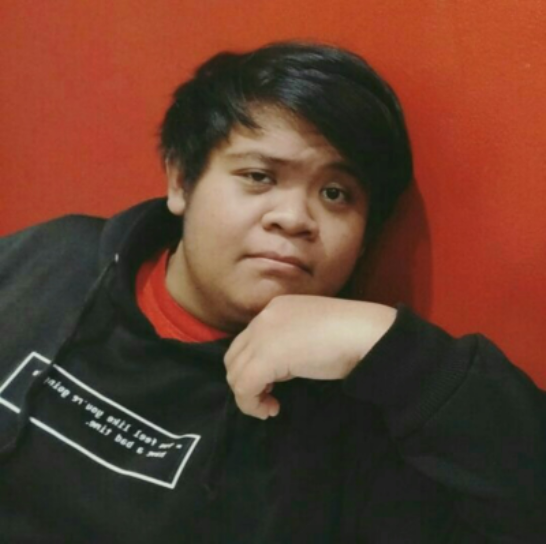
\includegraphics[width=0.3\textwidth]{gambar/profil.png}
  \vspace{-4ex}
\end{wrapfigure}

% Ubah kalimat berikut dengan biografi dari mahasiswa
Dimas Iqbal Fahreza atau yang lebih akrab disapa Dif, lahir di Bandar Lampung pada tanggal 6 Oktober 2000. Merupakan anak kedua dari dua bersaudara. Penulis lulus dari SMP Negeri 5 Yogyakarta dan kemudian melanjutkan ke SMA Negeri 2 Yogyakarta. Penulis merupakan salah satu mahasiswa dari Departemen Teknik Komputer Surabaya, Fakultas Teknologi Elektro dan Informatika Cerdas, Institut Teknologi Sepuluh Nopember. Dalam masa kuliah, penulis memiliki \emph{passion} terhadap bidang \emph{Game Development}. Selain itu, penulis juga memiliki hobi bermusik, baik dari memainkan alat musik piano, maupun membuat musik atau \emph{sound effects} untuk segala keperluan pengembangan gim. Penulis juga aktif ikut serta dalam kompetisi \emph{Game Development}. Kompetisi yang pernah dimenangkan adalah juara 3 GameDev HOLOGY 3.0. UB, dan menjadi finalis di MAGE ITS. Hingga sampai detik buku ini disusun, penulis masih memperjuangkan \emph{passion}-nya di bidang \emph{Game Development} dengan mengembangkan sebuah gim \emph{indie} pada tim yang telah didirikan sejak tahun 2021.
